%
%  Created by Kasper Nybo Hansen on 2011-05-22.
%  Copyright (c) 2011 Kasper Nybo Hansen. All rights reserved.
%
%
\documentclass[10pt]{article}

\RequirePackage{nybohansenPreamble}

\newcommand{\authorName}{Kasper Nybo Hansen}
\newcommand{\authorEmail}{nybo@diku.dk}
\newcommand{\titleName}{Exam Notes}
\newcommand{\courseName}{Advanced Algorithms}

\author{\authorName \\\texttt{\small{\authorEmail}}}
\title{\textsc{\titleName \\ \courseName}}
% \date{}
\makeindex

\begin{document}

\maketitle 

\tableofcontents

\section{Max Flow} % (fold)
\label{sec:max_flow}

The problem of max flow is finding a flow in a directed graph from a source to a sink. In the case of multiple sources and sinks, one can extend the graph by introducing a \emph{super source} and a \emph{super sink}.

\subsection{Definitions} % (fold)
\label{sub:definitions}
Let $G = (V,E)$ be a directed graph containing a source vertex $s \in V$ and sink vertex $t \in V$. Let every node $v \in V$ be reachable from $s$ and let $t$ be reachable from every node $v \in V$. Let each edge $(u,v) \quad \forall u,v \in V$ have a capacity $c(u,v) \geq 0$. The a flow is a real-valued function $f: V \times V \leftarrow R$, satisfying the capacity constraint and the flow conservation property. The capacity constraint says that the flow of an edge cannot exceed the capacity i.e
\begin{equation}
  0 \leq f(u,v) \leq c(u,v)
\end{equation} 
and the flow conservation property says that the total flow going into a vertex $u$ must be equal to the total flow going out of the vertex $u$, where $u \in V \setminus \{s,t\}$ i.e
\begin{equation}
  \sum_{v \in V} f(v,u) = \sum_{v \in V} f(u,v) \qquad u \in V \setminus \{s,t\}
\end{equation} 
The flow value, $|f|$, is calculated as
\begin{equation}
  |f| = \sum_{v \in V} f(s,v) - \sum_{v \in V} f(v,s)
\end{equation}
i.e. the flow value is calculated as the total flow going out of the source vertex minus the total flow going in.
% subsection definitions (end)

\subsection{Residual network} % (fold)
\label{sub:residual_network}
Let $f$ be a feasible flow in $G = (V,E)$. Let $G_f$ denote the residual network of $G$ induced by $f$, and let $f'$ be a flow in $G_f$. Then the function 
\begin{equation}
  (f \uparrow f')(u,v) = f(u,v)+f'(u,v)-f'(v,u) \qquad \forall (u,v) \in E
\end{equation}
denotes the augmentation of flow $f$ by flow $f'$.

It can be shown that $f \uparrow f'$ is a flow in $G$ and that the value is $|f \uparrow f'| = |f| + |f'|$.
% subsection residual_network (end)

\subsection{Cut} % (fold)
\label{sub:cut}
Given a graph $G = (V,E)$ a cut is a partitioning such that $V$ is divided into two subset $X$ and $Y$. We define the flow across a cut as
\begin{equation}
  f(X,Y) = \sum_{x \in X} \sum_{y \in Y} f(x,y) - \sum_{x \in X} \sum_{y \in Y} f(y,x)
\end{equation} 
thus the flow value of a cut is the total flow going from one subset to the other minus the total flow going the other way.

Let $G = (V,E)$, $X  = \subset V$, $Y = V \setminus X$, $s \in X$ and $t \in Y$. The partition $(X,Y)$ is then called a cut. The \emph{net flow} is defined as $f(X,Y)$. The capacity of the cut is defined as

\begin{equation}
 c(X,Y) = \sum_{u \in X, v \in Y} c(u,v)
\end{equation}
thus the capacity of a cut, is the total capacity of all connections between the two subsets.

% subsection cut (end)

\subsection{Min-cut theorem} % (fold)
\label{sub:min_cut_theorem}
A Min-cut is a cut where the capacity over all cuts is minimized. We thus choose to partition the $V$ such that the capacity, $c(X,Y)$, between the two sets are minimized.

Show that an augmenting path increases the flow value.

Show that the flow value has an upper bound. Let $V$, in a graph $G = (V,E)$, be partitioned into two subsets, $S$ and $T$. The flow value then has a upper bound equal to the capacity of the cut. The following proves this statement
\begin{align*}
 |f| &= f(S,T)  \\ 
     &= \sum_{s \in S} \sum_{t \in T} f(s,t) - \sum_{s \in S} \sum_{t \in T} f(t,s) \\
     &\leq \sum_{s \in S} \sum_{t \in T} f(s,t) \\
     &\leq \sum_{s \in S} \sum_{t \in T} c(s,t) \\
     &= c(S,T)
\end{align*}

Given a graph $G = (V,E)$, the min-cut theorem states that the following three statements are equivalent


\begin{enumerate}
  \item $f$ is a maximum flow in G, i.e the flow value, $|f|$, is maximized
  \item There are no augmenting paths in the residual network, $G_f$
  \item $|f| = c(S,T)$ for some cut $(S,T)$ in $G$
\end{enumerate}


The proof is done in a circular fashion. We will start by showing $1 \Rightarrow 2$ by contradiction. 

\begin{proof}
Let $f$ be a maximum flow in $G$. Let there be an augmenting path in the residual network. Hence there is a nonzero flow $f'$ in $G_f$. Thus $f \uparrow f'$ is stictly greater than $f$. This is a contradiction compared to our initial belief that $f$ was a maximum.
\end{proof} 

We will now show $2 \Rightarrow 3$
\begin{proof}
Assume that there are no augmenting paths in $G_f$, i.e. there are no paths between $s$ and $t$ in $G_f$, and they are there disconected. Now partition $G$ into two subsets, $S$ and $T$, such that $S = \{v \in V: \text{There is a path from $s$ to $v$ in $G_f$}\}$ and $T = V\setminus S$. I.e. $S$ contains the vertices reachable from the source node $s$ in $G_f$. Then $(S,T)$ is a cut. We now want to show that the value of this cut is equal to $|f|$. 

Let $u \in S$ and $v \in T$. 

If the edge $(u,v) \in E$, i.e. $(u,v)$ is an edge going from $S$ to $T$, then the flow going through this edge must be equal to the capacity, i.e. $f(u,v) = c(u,v)$ otherwise $(u,v) \in E_f$ which would place $v$ in set $S$. 

If the edge $(v,u) \in E$, i.e. $(v,u)$ is an edge going from the $T$ to $S$, then we must have that $f(v,u)=0$, otherwise $c_f(u,v) = f(v,u)$ would be positive and therefore $(u,v) \in E_f$ which would place $v$ in set $S$.

Thus the flow of the cut is

\begin{align*}
 f(S,T) &= \sum_{u \in S} \sum_{v \in T} f(u,v) - \sum_{u \in S} \sum_{v \in T} f(v,u) \\
        &= \sum_{u \in S} \sum_{v \in T} f(u,v) - 0 \\ 
        &= c(S,T) 
\end{align*}
\end{proof} 


The final thing we need to show is $3 \Rightarrow 1$. We thus need to show that $|f| = c(S,T)$ implies that $|f|$ is maximized. 

\begin{proof}
  We have shown that a flow has a upper bound of $c(S,T)$ i.e. $|f| \leq c(S,T)$. This means that $|f|$ must be maximized when $|f| = c(S,T)$.  
\end{proof}

The min-cut is the dual of the max flow.

% subsection min_cut_theorem (end)
                                                          
\subsection{Ford-Fulkerson and Edmonds Karp} % (fold)
\label{sub:ford_fulkerson_and_edmonds_karp}
The Ford-Fulkersen method works as follows:
\begin{verbatim}
  Initialize all edges to have a 0 flow
  Construct the residual network G_f   
  while augmenting paths exists in G_f do
    Find an augmenting path in G_f
    augment f with the max value found in the augmenting path 
    Construct the residual network for the increased flow
  loop 
\end{verbatim}

An example of running the Ford-Fulkerson method can be seen on figure \ref{fig1}

\begin{figure}[ht]
\centering
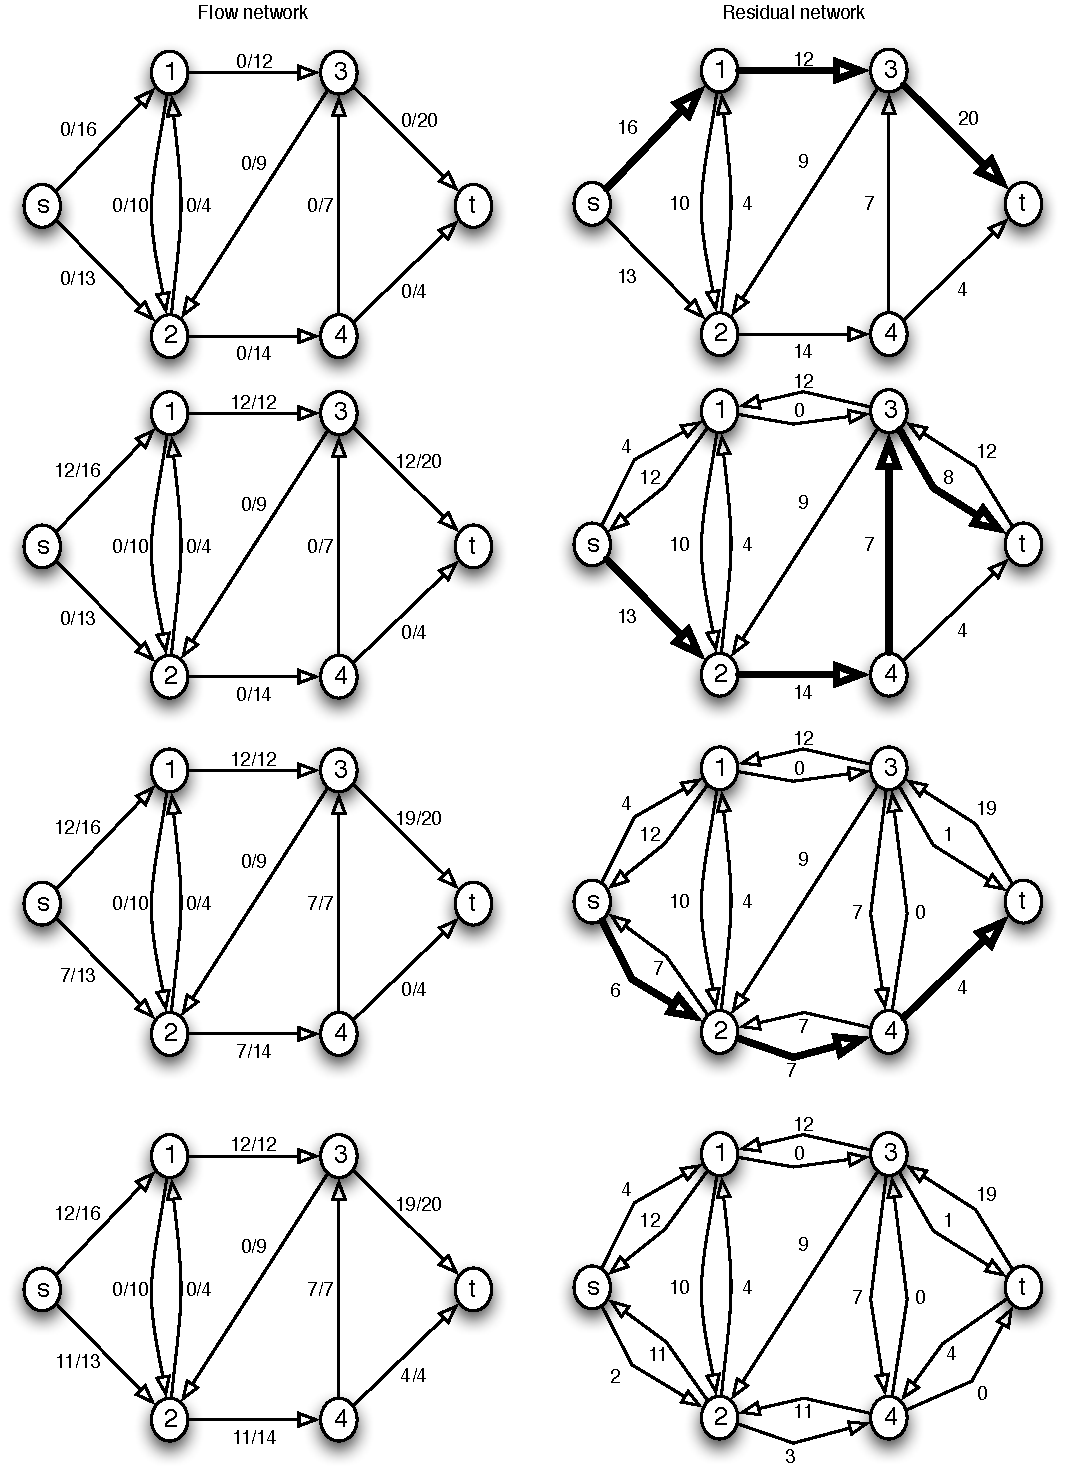
\includegraphics[width=0.9\textwidth]{figures/fig1.pdf}
\caption{Example of running the Ford-Fulkerson method. Left side is the flow network, right side is the residual network, with bold lines representing augmenting paths.}
\label{fig1}
\end{figure}

The running time of the Ford-Fulkerson can be expressed as $\O(E\dot f*)$ where $f*$ denotes the value of the max flow. At each iteration we search through $\O(E)$ edges, and the maximum number of iterations is $f*$. An illustration of this running time can be seen in figure \ref{fig2}.

\begin{figure}[ht]
\centering
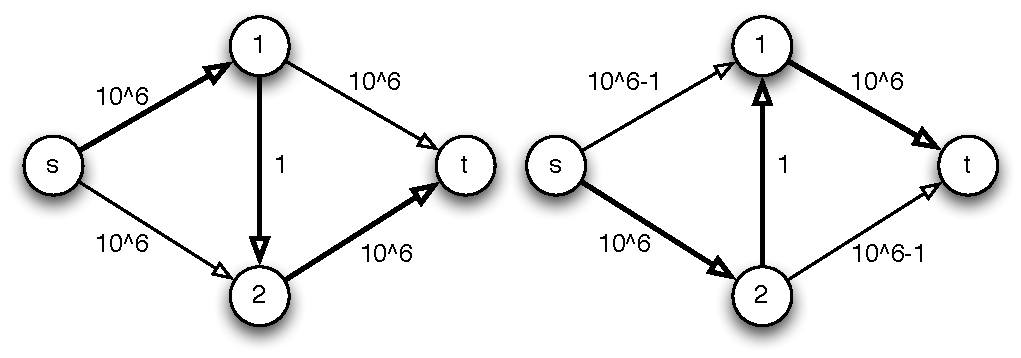
\includegraphics[width=0.9\textwidth]{figures/fig2.pdf}
\caption{Illustration of the complexity of the Ford-Fulkerson algorithm}
\label{fig2}
\end{figure}

This running time can be improved by selecting the augmenting path by breath first. Breath first chooses the shortest path with capacity between the source and sink. This is exactly what Edmonds-Karp does, thus Edmonds-Karp is a specialized version of the Ford-Fulkerson method. The running time of Edmonds-Karp is $\O(V^2E)$.


% subsection ford_fulkerson_and_edmonds_karp (end)

% section max_flow (end)

\section{Linear Programming} % (fold)
\label{sec:linear_programming}

In linear programming we want to maximize (or minimize) a linear function, under a number of constraints. An example of a linear program is
\begin{align}
 \max &\quad x_1 + x_2  \label{linprop1}\\ 
 \text{St.} &\quad  4x_1 - x_2  \leq 8 \nonumber\\
            &\quad  2x_1 + x_2  \leq 10 \nonumber\\
            &\quad  5x_1 - 2x_2 \leq -2 \nonumber\\            
            &\quad  x_1,x_2,x_3 \geq 0  \nonumber
\end{align}
\ref{linprop1} is called the objective function.
                                                                      
A linear program in 2 dimensions can be illustrated as figure \ref{fig3}. The gray area is called the feasible region.
\begin{figure}[ht]
\centering
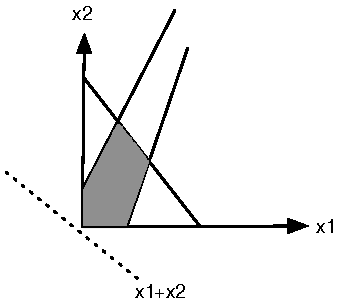
\includegraphics[width=0.5\textwidth]{figures/fig3.pdf}
\caption{Illustration of a simple linear program where the objective function is $x_1 + x_2$. The feasible region is gray.}
\label{fig3}
\end{figure}

A linear program can be written in two ways. Standard form and slack form. When a linear program is written in standard form it takes the following form
\begin{align*}
\max &\quad \sum_{j=1}^n c_jx_j  \\ 
 \text{S.t.} &\quad \sum_{j=1}^n a_{ij}x_j \leq b_i \qquad i=1,2,\ldots,m\\
             &\quad x_j \geq 0 \qquad i=1,2,\ldots,n\\
\end{align*}
where $m$ is the number of constraints and $n$ is the number of variables. One could think of $a$ as a matrix having, $m$ rows and $a$ columns. Every linear program can be rewritten to slack form. 

\subsection{Converting into standard form} % (fold)
\label{sub:converting_into_standard_form}
A linear program does not have to take standard form. But we can always turn a linear program into standard form. The following section describes how to convert a non-standard form linear program into standard form.

\begin{itemize}
  \item If the program is a minimization problem, then it can be turned into a maximization problem by multiplying the objective function by -1. The constraints are not changed, since the feasible region is the same, regardless if we want to maximize or minimize an objective function under the same constraints.                                                                         
  \item If the linear program contains variables, $x_j$ without nonnegative constraints we can replace $x_j$ so $x_j = x_j'-x_j''$, and add the constraints $x_j', x_j''>0$.
  \item If the linear program contains equality constraints, then replace each equality with to inequality constraints going opposite ways, i.e $a = b \Leftrightarrow a \leq b \wedge a \geq b$. 
  \item If the linear program contains inequality constraints, but instead of less than, they are greater than, then multiply the constraint with $-1$.
\end{itemize}

The following is an example of how to convert a non-linear program into standard form. 
\begin{align*}
 \min &\quad -2x_1 + 3x_2  \\ 
 \text{St.} &\quad  x_1 + x_2  = 7 \\
            &\quad  x_1 - 2x_2 \leq 4 \\
            &\quad  x_1        \geq 0  
\end{align*}

Start by making it a maximization problem, i.e. multiply the objective function with $-1$.
\begin{align*}
 \max &\quad 2x_1 - 3x_2  \\ 
 \text{St.} &\quad  x_1 + x_2  = 7 \\
            &\quad  x_1 - 2x_2 \leq 4 \\
            &\quad  x_1        \geq 0  
\end{align*}
Next place $x_2$ under the nonnegative constraint. Let $x_2 = x_2'-x_2''$ then
\begin{align*}
 \max &\quad 2x_1 - 3x_2' +3x_2''  \\ 
 \text{St.} &\quad  x_1 + x_2'-x_2''  = 7 \\
            &\quad  x_1 - 2x_2' +2x_2'' \leq 4 \\
            &\quad  x_1, x_2', x_2''    \geq 0  
\end{align*}
Make a cleanup so we remove those pesky primes, just rename $x_2' = x_2$ and $x_2'' = x_3$.
\begin{align*}
 \max &\quad 2x_1 - 3x_2 +3x_3  \\ 
 \text{St.} &\quad  x_1 + x_2-x_3  = 7 \\
            &\quad  x_1 - 2x_2 +2x_3 \leq 4 \\
            &\quad  x_1, x_2, x_3    \geq 0  
\end{align*}
Lets remove the equality sign, by replacing the equality with to opposite directed inequalities i.e.
\begin{align*}
 \max &\quad 2x_1 - 3x_2 +3x_3  \\ 
 \text{St.} &\quad  x_1 + x_2-x_3  \leq 7 \\
            &\quad  x_1 + x_2-x_3  \geq 7 \\
            &\quad  x_1 - 2x_2 +2x_3 \leq 4 \\
            &\quad  x_1, x_2, x_3    \geq 0  
\end{align*}
Final thing we need to do, is to turn the greater than into a less than my multiplying with $-1$, i.e.
\begin{align*}
 \max &\quad 2x_1 - 3x_2 +3x_3  \\ 
 \text{St.} &\quad  x_1 + x_2-x_3  \leq 7 \\
            &\quad  -x_1 - x_2 + x_3  \leq -7 \\
            &\quad  x_1 - 2x_2 +2x_3 \leq 4 \\
            &\quad  x_1, x_2, x_3    \geq 0  
\end{align*}
and the linear program in now in standard form.
% subsection converting_into_standard_form (end)


\subsection{Slack form} % (fold)
\label{sub:slack_form}
In slack form, the inequalities are replaced by equalities and a number of slack variables are introduced. We can rewrite the the standard form linear program shown in \ref{linprop1} to slack form as
\begin{align*}
 \max &\quad x_1 + x_2  \\ 
 \text{St.} &\quad  x_4 = 8 - 4_x1 + x_2 \\
            &\quad  x_5 = 10 -2x_1 - x_2\\
            &\quad  x_6 = -2 -5x_1 + 2x_2 \\            
            &\quad  x_1,x_2,x_3,x_4,x_5,x_6 \geq 0 
\end{align*}
% subsection slack_form (end)

\subsection{SIMPLEX algorithm} % (fold)
\label{sub:simplex_algorithm}
There exists several methods to solve linear programs. Some methods are polynomial, but doesn't work well in practice. A non polynomial method is called simplex. Simplex has it name from the shape of the feasible region.

Simplex needs the problem in standard form
% subsection simplex_algorithm (end)

\subsection{Duality} % (fold)
\label{sub:duality}
Weak and strong

What is it?

What is to be proved

Do not do the proof, but understand!


% subsection duality (end)

% section linear_programming (end)

\section{NP-completeness} % (fold)
\label{sec:np_completeness}
NP-completeness -CLRS, Chapter 34,   


The proof of  Theorem 34.13 was not treated in the lecture, and therefore it is given lower priority. You will not be asked to give an account for this proof in the exam. All other NP-completeness proofs in Chapter 34 have been covered, so it is recommended that you study and try to understand them. The "proof" of Lemma 34.6 (CIRCUIT-SAT is NP-hard) in the book is actually only a sketch of a proof, rather than a full proof, but it is worthwhile to study and understand the arguments which are given there. Further, of course you should know how the classes NP and Co-NP are defined, their corresponding languages, what it means that a problem is NP-complete, the notion of a reduction, etc.

% section np_completeness (end)

\section{Branch and Bound and Metaheuristics} % (fold)
\label{sec:branch_and_bound_and_metaheuristics}
Branch and Bound and Metaheuristics are  distributed notes ([Clausen] sections 1 and 2], [Luke] sections 0,1 and 2, [Fomin and Kratsch] chapter 1 and chapter 2).                                                                                                                                                          
% section branch_and_bound_and_metaheuristics (end)

\section{Approximation Algorithms} % (fold)
\label{sec:approximation_algorithms}


Approx Exam
Vertex cover appeox 2

Tsp approx 2 with triangle eq. Interesting if triangle not holds
Non approx algo if triangle not holds

Set cover

Good example Also to show how linear programme Can solcve set cover

Vertex cover, TSP, Set cover algorithm

Approximation Algorithms - CLRS, Chapter 35

Notes taken in class:
Approximate vertex cover an alternative way. Linear programming can be used in approx. algorithms. We want to solve vertex cover in a "weighted" version, called weighted vertex cover. Instead of wanting to archive the minimum number of nodes, we want to archive the minimum weight of the nodes.

Let every node $v_n$ have a weight $w(v_n)$. Goal: To minimize the total weight $\sum_{\forall v \in V} w(v)$ in the vertex cover. 


We need to express the problem in terms of integer programming. Thus
\begin{equation}
\sum_{\forall v \in V} w(v) x(v)  
\end{equation}
where $x(v)=1$ if vertex is in cover in cover otherwise 0. Subject to
\begin{equation}
  x(u)+x(v) \geq 1 \forall (u,v) \in E
\end{equation}
(At least one of two adjacent vertices has to be in vertex cover.) and
\begin{equation}
    x(v)  \in \{0,1\} \forall v \in V 
\end{equation}

We need to transform the integer programming problem into a linear program by relaxing the last constraint, i.e. $0 \leq x(v) \leq 1 \qquad \forall v \in V$. This linear program can be solved optimal in polynomial time. 

The solution of the linear program related to the solution to the integer problem-> Linear program gives us at leas the value of the integer programming problem. Linear program therefore gives us a lower bound.

Approx Exam
Vertex cover appeox 2

Tsp approx 2 with triangle eq. Interesting if triangle not holds
Non approx algo if triangle not holds

Set cover

Good example Also to show how linear programm Can solcve set cover

3CNF?!               

The whole chapter 35 has been treated in the lecture, except for the details of the proof of the approximation factor achieved by the greedy SET-COVER (pages 1120 and 1121), and except for the detailed computations in the proof of Theorem 35.8 (for  SUBSET SUM, pages 1132 and 1133).

For the approximation ratio for the greedy SET-COVER algorithms, another simpler proof was given during the lecture. It is based only on the number of remaining uncovered elements which are covered by the next set  selected by the greedy algorithm. Namely, if r is the number of remaining uncovered elements, the next set selected by the greedy algrorithm covers at least r/OPT elements, where OPT denotes the number of sets in the optimal solution (i.e. the minimum). This argument alone suffices to conclude that when the greedy algorithm selects at most OPT sets,  at least half of the remaining uncovered elements are covered. Repeating this argument recursively, yields that all elements are covered after selecting greedily at most OPT times $\O(log n)$ sets. For the purposes of the exam, it would suffice if you understand this argument (especially if you think that the full proof in the book is too difficult).

Similarly, in the exam you will not be required to give an account for the detailed computations in the proof of Theorem 35.8 (SUBSET-SUM), but you should try to understand the idea behind how trimming of the lists is done, and why it works. That is,

(a) on one hand it keeps only a polynomial number of elements in the list, but

(b) at the same time the allowed error is so small, that although it may increase at each step, it still does not add to something which is so big that it violates the required approximation bound.

% section approximation_algorithms (end)

\section{Randomized Algoritms} % (fold)
\label{sec:randomized_algoritms}
Randomized Algoritms - CLRS, Sections  5.1, 5.2, 5.3; 7.3, 9.2, 12.4, 35.4 (first part); (without the details of the probabilistic proofs in 7.3, 9.2 and 12.4)                                                                                                                                                    

Some problems can be solved in a simple way by using randomization. E.g. median finding. 

In median finding there is a linear algorithm that finds it deterministic, but a randomized algorithm is actual more efficient.

Affordability: Walking in a maze, in an "oblivious" manner i.e. we don't remember where we have been/walked until a certain point. At any node flip a coin to determine the direction. By doing this enough times you're guaranteed to sooner or later to arrive at the destination/goal. Such walks are called "random walks". 


Hiring problem: A way to model certain procedures, so can determine the worst case, expected cost and how we can use randomization to avoid worst case.


We want to hire a person. We have $n$ candidates. We interview each candidate, and if candidate $i$ is better than the previous best, we hire him.

The worst case is we hire all candidates, cost is thus $n$.

Expected hiring cost preciesly after the i'th interview is $1/i$

Expected total cost is $1+1/2+1/3+...+1/n \approx ln(n)$.

In order to arrive at this result we used the \emph{linearity of expectations}. Linearity of expectations means that the expected value of a sum equals the expected value of each i'th terms of the sum. Dice example.Throwing a dice yields a number in the interval $1-6$. The expected number is $3,5$. Throw the dice 10 times then the expected sum will be 35. This holds only for summation not products. For products it only holds for unrelated events (iid).

The worst case can be avoided by shuffling the list of candidates in a random permutation.


----------------

For the exam you should read and try to understand Sections 5.1, 5.2 and 5.3, the material for the randomized algorithm for MAX-3-CNF in Section 35.4, and give an idea of applications of randomization to sorting (Quicksort, Section 7), Selection (Section 9.2), and binary search trees (Section 12.4).You will not be required to give proofs for expected bounds for Quicksort, Selection and binary search trees, but you should try to give an intuitive explanation for how/why randomization works in these cases.

You will not be required to give the full proofs of Lemma 5.4 and 5.5 as they are given in the book (unless you want it), but you should try to convince yourself that these Lemmas are true and try to be able to argue about it. 



% section randomized_algoritms (end)

\section{Computational Geometry, Convex hulls} % (fold)
\label{sec:computational_geometry_convex_hulls}
Computational Geometry, Convex  hulls, CLRS,  Chapter 33.3 and the papers by [Kirkpatrick\&Seidel] and [Chan] (only 2D case in both articles).

Given a set of points $P$, the convex hull problem seeks to find a convex set containing all the points in $P$.

Let $S$ be a convex set. Then for any two points $a,b \in S$ the following is true
\begin{equation}
  (t-1)a+tb \qquad t \in [0,1]
\end{equation}
thus, there exists a line between any two points in $S$, such that the line between them is contained within $S$.

In the following we assume that no points has the same $x$- or $y$- coordinates and no three points are collinear. This is true in the continous world, but watch out when going into the discrete world of computers!

We denote the convex hull of a set $S$ to be $CH(S)$. There exists several algorithms to calculate the convex hull. Int he following, Grahams scan, Jarvis' march, quickhull, randomized incremental and marriage before conquest is explained in detail.

\subsection{Grahams scan} % (fold)
\label{sub:grahams_scan}
Grahams scan has a running time of $\O(n\log(n))$. It starts by choosing a the point $p_0 \in S$, with the lowest $y$-coordinate. This can be done in $\O(n)$. It then sorts the remaining points $p_i \in S$ by the angle between the line $(p_0, p_i)$ and the $x$-axis. This sorting can be done in $n \log(n)$ by e.g. heap sort\footnote{Heap sort uses a heap, i.e. a tree datastructure where the largest element is on top.} 

Put $p_0, p_1, p_2$ in the list of nodes that constitutes the convex hull. If making a left turn when adding $p_3$, remove $p_2$ and add $p_3 to the list$. Otherwise if making a right turn, add $p_3$ to the list. Continue adding nodes. If adding node $p_j$ creates a left turn, then remove node $p_{j-1}$ and add $p_j$. Otherwise just add $p_j$. When last node has been reached, the convex hull is done.

The correctness of Grahams scan can be explained by the following observations. 

\begin{itemize}
  \item Grahams scan will never go backwards behind the initial node. 
  \item When ariving at point $p_i$ all points between the initial node and the point $p_i$ are right turns on the polygonal line constructed so far
  \item After arriving at the initial node by a right turn, we get a polygonal line consisting of purely right turns. 
\end{itemize}



The time complexity is $\O(n\log(n))$ since sorting takes $\O(n\log(n))$ and the scanning takes $\O(n)$, since each point is only considered once. The total time complexity is thus $\O(n\log(n)+n)=\O(n\log(n))$.

% subsection grahams_scan (end)

\subsection{Jarvis' march} % (fold)
\label{sub:jarvis_march}
Jarvis' march is also knows as the `Giftwrapping algorithm'. It has a complexity of $\O(nh)$, where $n$ is the number of nodes, and $h$ is the number of nodes in the convex hull. Since part of the complexity relies on the final output, the algorithm is \emph{output sensitive}.

Find the point, $p_0$, which is placed leftmost. This point can be found in $\O(n)$. Add $p_o$ to the convex hull list. Now find the point $p_1$ which has every other point $p_i$ to the right and add it to the list of convex hull nodes. This can also be done in $\O(n)$ by comparing polar angles from $p_0$. Continue to add $p_i$ to the list such that every other node is to the right of $p_i$. Continue until the $p_i=p_0$.

The complexity of Jarvis' march can be computed as the time it takes to find $p_i$ times the number of nodes, $h$ in the convex hull. The complexity is thus $\O(nh)$.
% subsection jarvis_march (end)


\subsection{Quickhull} % (fold)
\label{sub:quickhull}
Quickhull is an algorithm that has an expected running time of $\O(n\log(n))$, and a worst case running time of $\O(n^2)$. The algorithm starts by finding the leftmost and rightmost points, $A$ and $B$. It then draws a line between these two points, and splits the point set $S$ into two. Let the set $S_1$ contain the points above the line, and $S_2$ contain the points below the line. 

For each of these two sets we proceed recursively.

Find the point, $P$ farthest away from the line. the convex hull must contain $P$, so insert the point between $A$ and $B$. A triangle is formed by $ABP$. Remove all points from $S$ that is contained within this triangle. The cross product can be used to calculate wether a point lies inside a triangle.                                                                                        

We form two new sets. One set containing the set of points above the line $AP$. The other set containing the line $BP$. The line $AB$ is then replaced by these two lines. and the algorithm proceeds recursively. The algorithm stops when the sets are empty or if it only consist of one node.

If the partitioning yields balanced sets, the the expected running time is $\O(n\log(n))$. If the partitioning is extremely unbalanced then the running time is $\O(n^2)$. A example of an extremely unbalanced set of points, is when the points lie on a half circle.


% subsection quickhull (end)

\subsection{Marriage before conquest (MBC)} % (fold)
\label{sub:marriage_before_conquest_mbc_}
The Kirkpatrick-Seidel algorithm (Marriage before conquest) is output sensitive and has running time $\O(n\log{h})$, where $h$ is the number of points in the convex hull.

The algorithm first calculates the upper hull and then the lower hull. It then merges these two into the final convex hull. We can safely assume that the merging of the two half hulls can be performed in $\O(1)$.

Let $S$ be the set of points. Divide $S$ into two sets, by dividing $S$ with the line $(p_j,p_k)$, where $p_j \in S$ is the point with minimum $x$-value and $p_k \in S$ is the point with maximum $x$-value. Let $P$ be one of the two sets.

The algorithm then calculates the median $x$-coordinate $M$ of the points in $P$. It the finds the bridge segment that crosses the vertical line $x=M$. It finds this bridge segment by a technique called Prune \& Search. $x=M$ divides $P$ in half. The bridge segment across this line, will be part of the final convex hull. Finding the bridge is done by the following procedure.

Randomly pair the points in $P$ into $n/2$ distinct line segments. Name the line segments $q_i$. Let the point of line segment $q_i$ with the lowest $x$-value be called $q_{il}$, and the point with the largest $x$-value $q_{ir}$. This pairing can be done in $\O(n)$.

Determine the median slope, $m$ of all the distinct line segments. If the number of points is odd, there will be a point that is not part of a line segment. Give this point a slope of $0$. If the number of line segments is even there are two choices for the median slope. Let $m$ be the max of these two slopes.

Construct a sweep line, $L$, having the median slope, i.e $y = mx+b$. Find a point $p_t$ such that $L$ is a supporting line\footnote{A supporting line for a set $S$ is a line that contains a point $p_i \in S$ an no other points above.} for $P$ at $p_t$, this can be done by translating. We call $p_t$ the top point. Let $p_j.x$ define the $x$-coordinate of the point $p_j$. If $p_t.x \geq M$, i.e the top point is to the right of the vertical line M, then for each line segment with slope $< m$ remove the right point of the line segment, i.e $q_{ir}$. If $p_t.x < M$, i.e. the top point is to the left of the vertical line $M$, then for each line segment with slope $>m$, remove the left point $q_{il}$. Repeat this until only two points are left. We know that at least half of the line segments has a slope greater than $m$, therefore we can conclude that we at each iteration of the bridge finding removes $1/4$ of the points. Note that the points are only removed in the current step where we find the bridge, not the set $P$.

Delete the points under the bridge, and split $P$ into the two half's divided by the vertical line. Continue recursively on each half.

The complexity of the bridge finding is as follows. Pairwise point matching takes $\O(n)$, finding the median slope takes $\O(n)$, slope translation takes $\O(n)$. Each time we remove points we are sure to remove $1/4$ of the points. This yields 
\begin{align*}
T(n) &= \O(1) &\qquad n=2\\ 
T(n) &= T(3n/4) + \O(n) &\qquad \text{if } n>2
\end{align*}
thus the complexity of the bridge finding and finding the median is $T(n)=\O(n)$.

The total overall complexity can be bounded by the following function
\begin{align*}
f(n,h) &= cn &\qquad h=2  \\ 
f(n,h) &= cn + \max_{h_l+h_r = h}\left\{f(n/2,h_l)+f(n/2,h_r)\right\} &\qquad h>2
\end{align*}
where $c$ is a positive constant. The max is introduced because the algorithm is output sensitive. The claim is that the complexity is $f(n,h) = \O(n\log(h))$, thus we can find a upper bound by the function $cn\log(h)$.

\begin{proof}

  For $h=2$                
  \begin{equation}
    f(n,h) = c_1n \leq cn\log(2)
  \end{equation}
  this trivially holds if $c_1 \leq c$
  
  Assume $h>2$ and bu subsitution we have
  \begin{align*}
   f(n,h) &= cn + \max_{h_l+h_r = h}\left\{cn/2\log(h_l)+cn/2\log(h_r)\right\} \\
          &= cn + cn/2\max_{h_l+h_r = h}\left\{\log(h_l)+\log(h_r)\right\} \\
          &= cn + cn/2\max_{h_l+h_r = h}\left\{\log(h_lh_r)\right\} \\          
          &= cn + cn/2\max_{h_l+h_r = h}\left\{\log(h_l(h-h_l))\right\} \\         
          &= cn + cn/2\max_{h_l+h_r = h}\left\{\log(hh_l-h_l^2))\right\}                    
  \end{align*}
    
  When does the function $g(h_l) = \log(hh_l-h_l^2)$ takes it's maximum. It does when the derivative is $0$.
  \begin{equation}
    g_{h_l}'(h_l,h) = \frac{1}{hh_l-h_l^2} (h-2h_l) = 0 
  \end{equation}
  If $g_{h_l}'(h_l)=0$ then $h-2h_l=0$ yielding $h_l = \frac{h}{2}$. Thus
  \begin{align*}
   f(n,h) &= cn + cn/2\log(h\frac{h}{2}-\frac{h^2}{2^2})) \\
          &= cn + cn/2\log(\frac{h^2}{2}-\frac{h^2}{2^2})) \\   
          &= cn + cn/2\log(\frac{2h^2}{4}-\frac{h^2}{2^2})) \\
          &= cn + cn/2\log(\frac{h^2}{2^2})) \\                       
          &= cn + 2cn/2\log(\frac{h}{2}) \\                                 
          &= cn + cn\log(\frac{h}{2})                                 
  \end{align*}
   which has a running time of $\O(n\log(h))$
   
\end{proof}

% subsection marriage_before_conquest_mbc_ (end)

% section computational_geometry_convex_hulls (end)




\section{Computational Geometry, Delaunay triangulatiom} % (fold)
\label{sec:computational_geometry_delaunay_triangulatiom}
Computational Geometry, Delaunay triangulations (and Voronoi diagrams): From the  book Computational Geometry, Algorithms and Applications, Chapter 9,  Sections 9.1, 9.2, 9.3, available at http://www.cs.uu.nl/geobook  without the proofs.                                                                  
% section computational_geometry_delaunay_triangulatiom (end)




\end{document}